\documentclass[12pt]{article}
\usepackage{amsfonts, epsfig}
\usepackage[authoryear]{natbib}
\usepackage{graphicx}
\usepackage{fancyhdr}
\pagestyle{fancy}
\lfoot{\texttt{ematm0067.github.io} / \texttt{ematm0044.github.io}}
\lhead{Introduction to AI - 01.1\_introduction - Conor}
\rhead{\thepage}
\cfoot{}

\usepackage{tikz}
\usetikzlibrary{positioning}

\usepackage{ifthen}
\newboolean{nopics}
\setboolean{nopics}{true}


\begin{document}

\section*{What is this unit about?} 
This unit is about machine learning and artificial intelligence;
effectively this means it is about how we can automate the processes
of drawing inference from data. In a way this description of the unit
is uncontroversial; that is certainly what machine learning attempts
to do, but it is also confusing in the sense that that is one of the
main goals of all of science, Newton's Law allows us to infer the
consequence of a force on a mass, the rules discovered by geneticist
allow us to infer some parts of our fate from our genes. I suppose
that ML and AI can be thought of as an approach to inference that
relies strongly on data. Of course science has a broader ambition, it
hopes to explain our reality as well as describe it. This too is
something science shares with ML / AI; one of our ambitions for the
subject is that it explain something about the nature of computation
and the nature of intelligence.

ML / AI has, over the years, progressed in fits and starts and our
understanding of the subject has changed back and forth. Sometimes it
was considered useful to work in a very principled way, using very
explicit models of our data; we will see examples of this in this unit
when, for example, we look at linear regression. At other times, the
subject has been enthralled by the `unreasonable effectiveness' of
less principled methods; we are currently in the middle of such a time
with deep learning neural networks proving vastly more effective than
most had expected. We will look at example of this sort too, or,
rather, we will have a look at some neural networks. It is important
in studying the subject to learn about a whole variety of approaches
and not to consider one correct and the other wrong, the history of
our discipline has taught us to move forward as a sailboat does when
sailing against the wind, by tacking first one way and then other, but
always making progress. We are practical people and ML / AI is a
practical subject, our greatest loyalty should always be to what
works!


\section{Parts to this unit}

The first two parts of the unit deal with the classic subdivision of
machine learning into \textsl{supervised} and \textsl{unsupervised}
learning. Often times too much emphasis is put on this distinction, or
the distinction is made out to be more clear cut than it is; however,
it is a traditional and useful organising principle for units like
this. We will then consider neural networks; though they will have
already been mentioned as part of supervised learning. Looking at
these algorithms will have made it clear how they rely on data and how
this creates risks and challenges so the next part considers
ethics. Finally we will look at Bayesian approaches to data and at
some other algorithms related to search and agent-based modelling.

\subsection{Supervised learning}

In supervised learning we have data and some property of the data we
are interested in, perhaps medical records and the patient outcome or
pictures of animals and the sort of animal pictured. We hope to
develop to be able to generalise to data where we don't have information about the
property of interest. Put another way we have a set of pairs
\begin{equation}
  \mathcal{T}=\{(\mathbf{x}_i,y_i)\}
\end{equation}
where the $\mathbf{x}_i$ is the data describing the item $i$ and $y_i$
is the property of $i$ that is of interest. Often $\mathbf{x}_i$ is
called the \textsl{input} whereas $y_i$ is called the
\textsl{label}. The set of pairs $\mathcal{T}$ is the \textsl{training
  set}. The idea is to make a map:
\begin{equation}
  C(\mathbf{x}_i;\theta)=\tilde{y}_i
\end{equation}
where $\theta$ are some parameters describing the map. The training
set is used to fix these parameters so that $\tilde{y}_i$ is a good
approximation to $y_i$. The hope is that for novel data
$\mathcal{N}=\{\mathbf{x}_i\}$ the map will give a good prediction
for the corresponding, unknown $y_i$.

A very simple example might help, say your data are
\begin{equation}
  \mathcal{T}=\{(1,7),(-1,-1),(2,10)\}
\end{equation}
and you suspect the data are described by a line so $C(x;m,c)=mx+c$
where $m$ and $c$ are the parameters, summed up as $\theta$ above. The
training data can be used to work out the values of $m$ and $c$, in
fact $m=3$ and $c=4$, now if you are given a novel input, say $x=5$
you can predict that the corresponding label is $19=3\times 5+4$. This
example is intended to introduce the idea that the algorithms has some
parameters, $\theta=(m,c)$ that will need to be set by the training
data. However, as an example of data, it is a poor example because it
is so simple and because it has no noise.

Here is another example: you have lots of pictures of dogs and cats,
you know which are which and you train a classifier using these
data. Now, the hope is that the same classifier, if presented a
picture, will be able to make a good guess as to whether it is a cat
or a dog. As another example, you have MRI scans of patients with mild
cognitive impairment; MCI is sometimes a precursor to Alzheimer's
disease, sometimes it is harmless and the MCI improves, sometimes the
conditions leading to the MCI diagnosis are the result of healthy
aging and the subject continues to have MCI but does not have
Alzheimer's disease. It is becoming important, from a treatment
point-of-view to spot how MCI is going to resolve itself and, in
needed make a intervention without waiting to see what happens. If you
wait until the disease develops clearer symptoms the treatment is not
effective. In supervised learning you would like to take the MRI scans
from MCI patients examined in the past and your knowledge based on
follow-ups of whether the MCI progressed to Alzheimer's disease to
train a classifier so that, in future, you can use the brain scan to
decide on treatment while there is still time to help.

In this part of the unit we will consider $k$-nearest neighbours,
regression, na\"ive Bayes and simple neural networks.

\subsection{Unsupervised learning}

In unsupervised label there is no label, so it is the task of the
algorithm or machine to discover the structure of the data. This is
clearly useful; going back to the MCI example, collecting labelled
data is very difficult, you need to wait years to find out if patients
develop Alzheimer's disease. Imagine you have new measurements, some
sort of set of cognitive tests or brain scans, or blood measurement,
and want to guess whether it is useful. One approach would be to try
unsupervised labelling, to see if the subjects naturally fall into
groups using the data; if they do, you could investigate the different
groups further to see if there is any indication that one of the
groups is associated with disease.

However, unsupervised learning is hard, consider the example mentioned
above, a large collection of pictures of dogs and cats. In
unsupervised learning the algorithm would be presented with the set of
pictures and be tasked with finding the structure, in this case, the
grouping into cat pictures and dog pictures. Of course, there might be
other groupings that make since, large animals versus small animals,
brown and brown animals versus animals with a lighter color, animals
sitting down versus animals standing. In fact, unsupervised learning
is tricky and rarely as undirected as the name suggests, but it is
very useful, unlabelled data is easier to come by than labelled data,
and it is useful to think about unsupervised learning since it is
probable that the aspects of an algorithm that support unsupervised
learning are also present in the most powerful supervised algorithms.

It is interesting to consider that unsupervised learning must play a
role in human learning, we do learn from supervised or reinforced
examples, but a lot of the data we encounter is unlabelled. It is
likely we learn \textsl{representations} of data in part in an
unsupervised way and in part in a supervised way; by representations
we mean the way the data are mapped into a space of data so that their
encoding and location tells us something about their properties. These
days we think about machine learning as a process of producing good
representations mixed with inference on those representations; in
simple problems we do it without thinking, if we want to examine the
performance of sportsperson for example, we would consider plotting
them as points on a graph showing things like `attempts at goal' and
`goals scored'; the space (attempts at goal)-(goals scored) is a
representation.

In this part of the unit we will consider $k$-means clustering,
hierarchical clustering, competitive clustering, Gaussian clustering
along with component methods.

\subsection{Neural networks}

At its simplest a neural network can be thought of as a specific form
of map; in the supervised case, an most neural networks are used for
supervised learning, this is the map $C$ above from input
$\mathbf{x}_i$ to label $y_i$. In a neural network this map is
described in terms of a network of interacting nodes.
\begin{center}
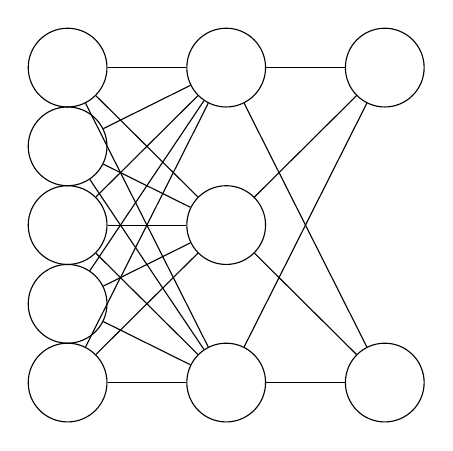
\begin{tikzpicture}[
    node distance=2.5cm and 1cm,
    neuron/.style={circle, draw, minimum size=1cm}
]

\def\in{5}
\def\hn{3}
\def\on{2}
  
% Layer 1
\foreach \i in {1,...,\in}
    \node[neuron] (L1-\i) at (0,-\i) {};

% Layer 2
    \foreach \i [evaluate=\i as \position using int(\in*\i/\hn)] in {1,...,\hn}
    \node[neuron, right=of L1-\position] (L2-\i) {};

% Layer 3
\foreach \i [evaluate=\i as \position using int(\hn*\i/\on)] in {1,...,\on}
    \node[neuron, right=of L2-\position] (L3-\i) {};

% Connections L1 to L2
\foreach \i in {1,...,\in}
    \foreach \j in {1,...,\hn}
        \draw (L1-\i) -- (L2-\j);

% Connections L2 to L3
\foreach \i in {1,...,\hn}
    \foreach \j in {1,...,\on}
        \draw (L2-\i) -- (L3-\j);

\end{tikzpicture}
\end{center}
In this picture the data is input as values for the left hand nodes
and these values are combined to give input to the middle nodes; the
lines represent multipling the input by some weight and then adding
them. In this picture the input to the middle node is something like
\begin{equation}
  h_2=\sum_{j=1}^5w_{2j}x_i+b_2
\end{equation}
where the $x_i$ are the input values and the $w_{ij}$ are weights and
$b_j$ is a sort of offset called a bias. The output of that node is
then a non-linear function of $h_2$. This is inspired by the
architecture of neuronal computation, that is, computation in the
brain, but can usefully be thought of as a way to make complicated
maps or functions. The weights and biases, the vast number of the
$w_{ij}$s and $b_i$s that go into the network are the learnable
parameters.

As you will have heard, there has over the last 15 years or so been a
huge success with using neural networks for AI / ML tasks.


\subsection{Ethics}

There are huge ethical challenges associated with AI / ML: most
obviously the wonderful effectiveness of modern learning algorithms
mean that the action of the algorithm is mysterious and opaque. This
bring with it the danger of unintended consequences, the possibility
that the algorithm with exaggerate or distort societial biases and
norms. This is made more problematic by their consequence, as AI / ML
is being used for real world decision making and inference we need to
know how to prevent that codifying negative aspects of our historic
attitudes which have become implicit in incidious ways in our data.

Certain the history of our subject has been marked with
ethical failures and some of its foundational figures have had
objectional views. Even the `iris' dataset, a commonly used example
collection of petal and sepal measurements used illustrate simple
linear models was first used in the context by Ronald Fisher, a
complex figure whose influence on data science is immense but whose
views, while disputed, where almost certainly discriminatory.

Beyond this, ethics in AL / ML needs to address complex questions of
ownership and reward. It is difficult to match the huge profits and
the huge power that is the likely reward of control of machine
learning technologies and the poorly rewarded and overlooked labour
that went into producing the data on which it feeds. As a sort of
trivial example about twenty years ago I became very involved in
creating wikipedia pages for Irish artists; I was happy to do this as
a free contribution to the community, should I know receive some small
monetary return for producing the data used to train large language
models? These are difficult questions and so it essential we consider
them.

\subsection{Other approaches}

In this part of the unit we consider other approaches to AI / ML such
as agent-based algorithms, search algorithms and Bayesian
models. These approaches are often useful for small data problems or
for specific applications and, while they have not had the broad
influence recently that deep learning neural networks have, they are
benefiting from the same advances in computing and in our
understanding of algorithms; for example, though we won't discuss it
here, Bayesian modelling is in the middle of a revolution of its own
with the discovery of Hamiltonian / Hybrid Monte Carlo. It seems
inevitable that the future of AI / ML will involve insight from these
other approaches to data and inference and, from a scientific
point-of-view, these approaches are often more closely aligned to
cognitive science.

\section{Summary}

In these notes we set out the scope and philosophy of the unit; there
are brief sketches of supervised and unsupervised learning and of
neural networks. The ethics section of the unit is
motivated. Everything here will be returned to in one form or another
as the unit progresses!

\end{document}

